%%%%%
% CH4 %
%%%%%

\chapter{Transient heat conduction}
	Let's Imagine that we want to cool a bottle of beer. What time will it take ? We will consider 3 different cases neglecting sometimes convection sometimes conduction. 
	
\section{Lumped systems analysis}
	\begin{wrapfigure}[6]{l}{3cm}
	\vspace{-5mm}
	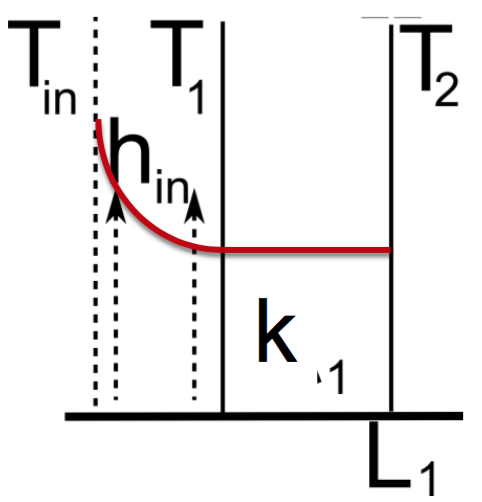
\includegraphics[scale=0.3]{ch3/8}
	\end{wrapfigure}	
	Let's study the case where convection is the limitative factor for heat (dispersion of heat within the solid is negligible compared to heat arrival to the surface). Let's remind the expression of the Biot number (go to \autoref{sec:3.3.3}). In this case, the $Bi \ll 1$
	\begin{equation}
		Bi = \frac{L_1h_{in}}{k_1}
	\end{equation}
	
	\subsection{Calculation of lumped systems}
		Let's consider an object of volume $V$ and surface $A$ initially to temperature $T_i$ that we put into an infinite temperature $T_\infty$ enviroment. We want to know what happens. So my accumulation, is equal to the amount that comes with the convection
		\begin{equation}
			V\rho c_p \frac{\partial T}{\partial t} = A h(T_\infty - T)
		\end{equation}
		Integrating and applying the initial condition $t = 0 \rightarrow T = T_i$
		\begin{equation}
			\underbrace{\frac{T-T_\infty}{T_i - T_\infty}}_{\theta} =
			 \exp \left( - \frac{Ah}{V\rho c_p}t \right) = 
			 \exp \left( - \underbrace{\frac{Vh}{Ak}}_{Bi} \underbrace{\frac{A^2k}{V^2\rho c_p}t}_{Fo} \right) 
		\end{equation}
It can always be expressed like a function of theta. 
The expression in the $\exp$ must be undimentional so we will make it appear. $V/A$ = lenght, so the definition of Biot number appears. The other is including t and is called the \textbf{Fourrier number}. 

	\subsection{Fourrier number}
		\begin{equation}
			\theta = \exp (-Bi \, Fo) \qquad Fo = \frac{A^2k}{V^2 \rho c_p}t = \frac{A^2\alpha }{V^2}t
		\end{equation}
		If we look to the units, we see that it's the undimentionnal time of the process. It compares the time since the external temperature change and the characteristic time of heat conduction in the object. 
		
\section{Semi-infinite solid}
	\subsection{Error function}
		\begin{wrapfigure}[7]{l}{2.8cm}
		\vspace{-5mm}
		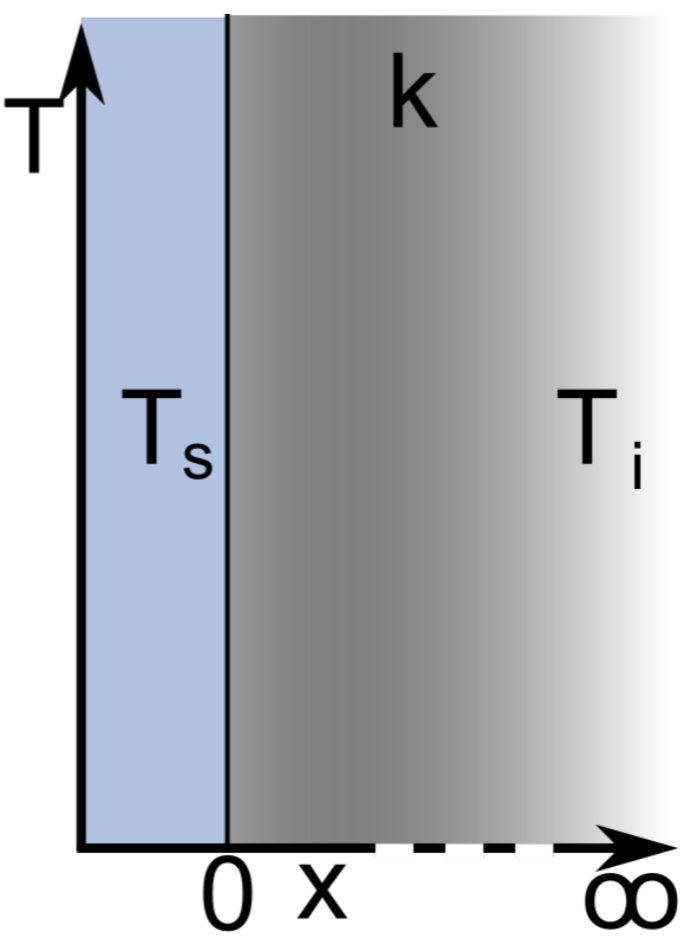
\includegraphics[scale=0.2]{ch4/2}
		\end{wrapfigure}	
		This is the case within the conduction only appear on a small franction of the total solid and an infinite surface is in contact with a fluid. The $Bi \gg 1$. We respect equation without source term 
		\begin{equation}
			\frac{\partial T}{\partial t} + \alpha \frac{\partial ^2 T}{\partial x^2 }
		\end{equation}
		We don't do the calculus in the course but after integrating and applying the conditions $T = T_S$ for $x=0$ $\forall t \leq 0$, $T = T_i$ for $x\rightarrow + \infty$ and $T = T_i$ for $t=0$ $\forall x > 0$, we obtain the result 
		\begin{equation}
			\frac{T-T_S}{T_i-T_S} = erf(\eta ) \qquad with \qquad \eta = \frac{x}{\sqrt{4\alpha t}} \qquad and \qquad erf(\eta ) = \frac{2}{\pi} \int _0 ^\eta \exp (-u^2) \, du
		\end{equation}
		
		\begin{wrapfigure}[7]{r}{2.8cm}
		\vspace{-5mm}
		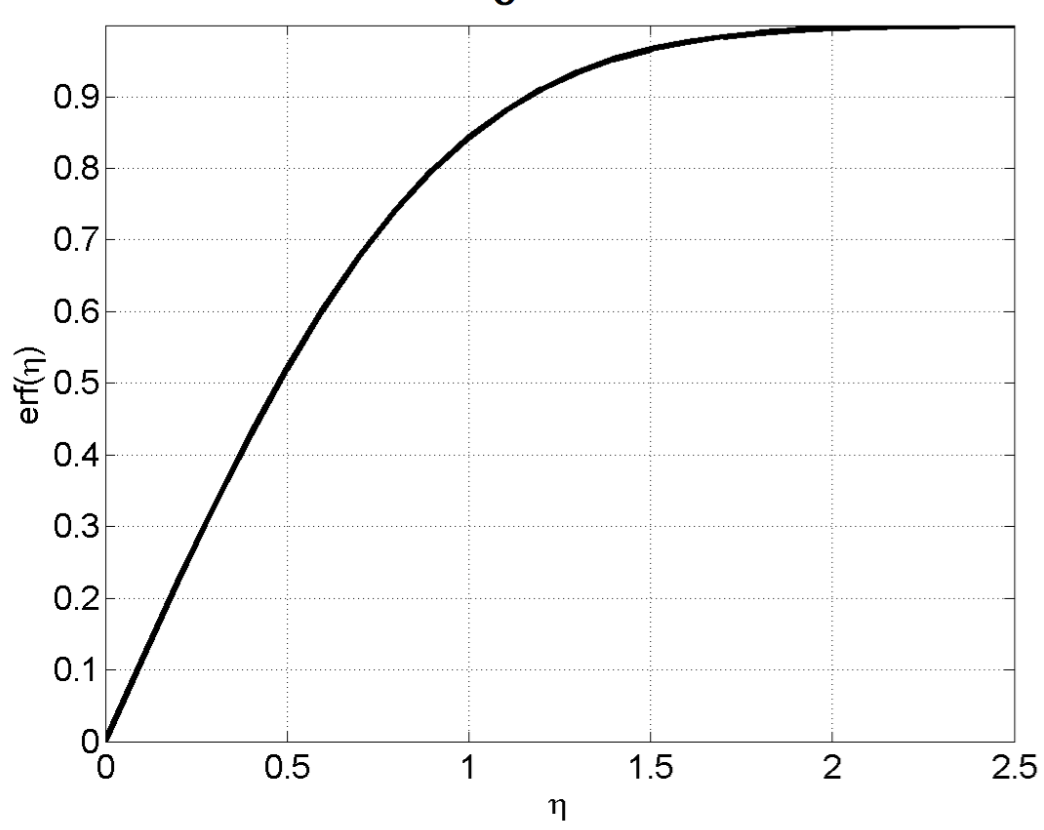
\includegraphics[scale=0.2]{ch4/3}
		\end{wrapfigure}	
		We see that $\eta$ combines position and times. You progress in the object proportionallly to the square root of time. A fixed value of $\eta$ means a fixed value of temperature. The flux density is expressed 
		\begin{equation}
			\dot{q} = -k \frac{\partial T }{\partial x }| _{x=0} = k \frac{T_S-T_i}{\sqrt{\pi \alpha t}}
		\end{equation}
Im assuming an infinite body, is it realistic ? where does my heat go ?

	\subsection{Penetration lenght}
		\begin{wrapfigure}[7]{l}{3.5cm}
		\vspace{-5mm}
		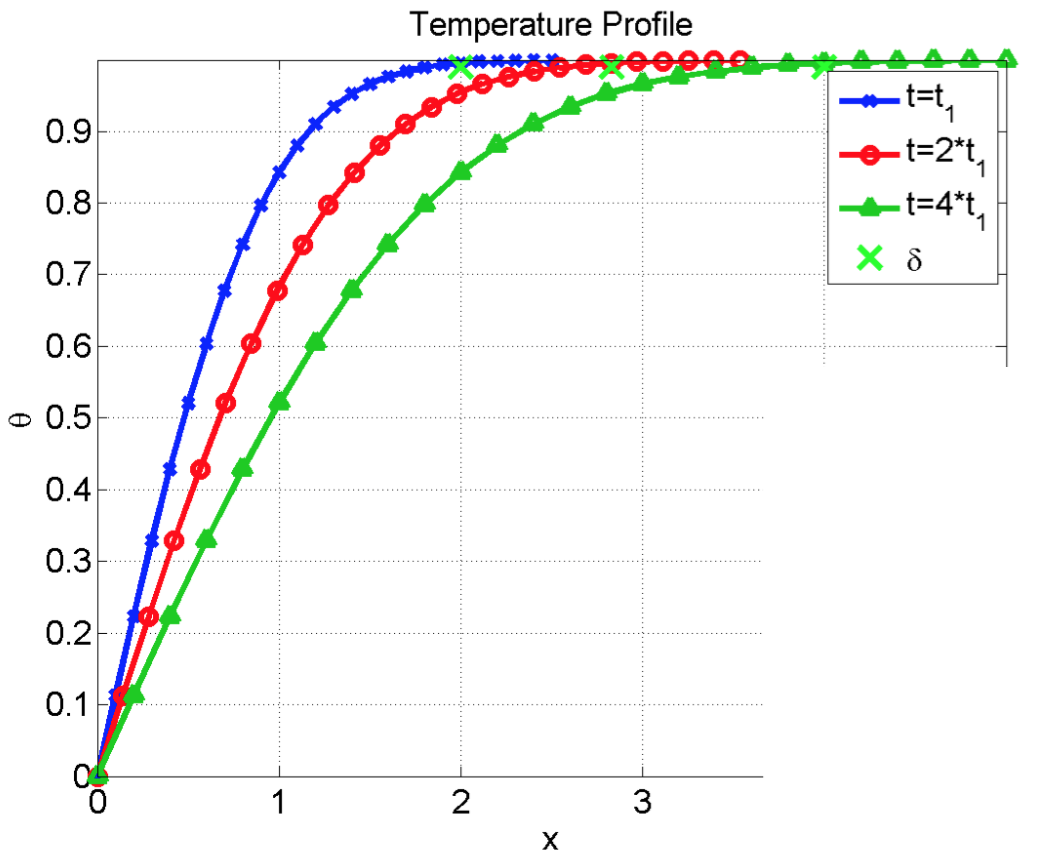
\includegraphics[scale=0.2]{ch4/4}
		\end{wrapfigure}	
		When we look to the graph, we can see that if the process time is 4 time higher, the $x$ goes 2 times further. We define the penetration length 
		\begin{equation}
			\delta = 4\sqrt{\alpha t}
		\end{equation}
		that defines the range of the heat process. \\
		But when is this applicable ? As long as the center of the object is not reached. Let's suppose a characteristic length $L$. We must respect the condition $\delta = 4\sqrt{\alpha t} < L$. After manipulations (Bi still $\gg 1$)
		\begin{equation}
			\frac{\alpha t}{L^2} = Fo < \frac{1}{16}
		\end{equation}
	
	\subsection{Two semi-infinite body in contact}
		\begin{wrapfigure}[7]{r}{3cm}
		\vspace{-5mm}
		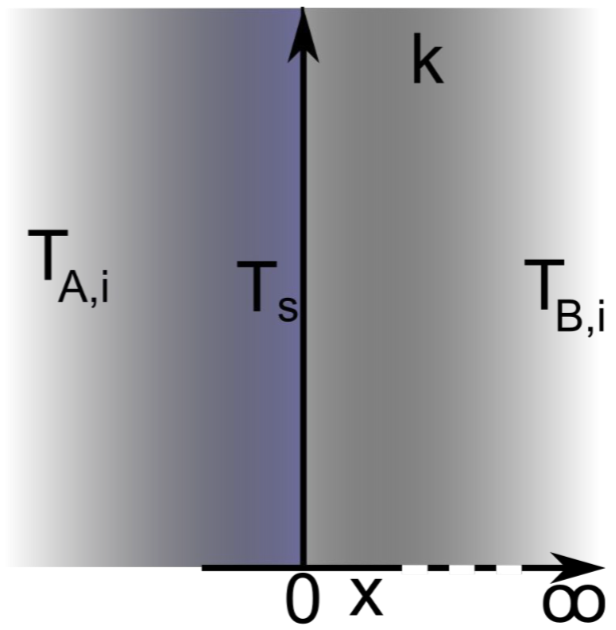
\includegraphics[scale=0.3]{ch4/5}
		\end{wrapfigure}	
		What happens when two solids enter in contact ? If the time is short enough ($Fo < 0.16$), we can consider the 2 as semi-infinite bodies. So (for heat comming from B)
		\begin{equation}
			\dot{q}_{s,A} = \dot{q}_{s,B} \Leftrightarrow k_A \frac{T_S-T_{Ai}}{\sqrt{\pi \alpha _A t}} = k_B \frac{T_{Bi}-T_S}{\sqrt{\pi \alpha _B t}}
		\end{equation}
		After isolating $T_S$ and expressing $\alpha$ as \autoref{eq:3.7}
		\begin{equation}
			T_S = \frac{\sqrt{K_A C_{pA}\rho _A}T_{Ai} +\sqrt{K_B C_{pB}\rho _B}T_{Bi}}{\sqrt{K_A C_{pA}\rho _A}+\sqrt{K_B C_{pB}\rho _B}}
		\end{equation}
		This is an average temperature indepedendent of time. \\
		We cannot apply that theory in the case of our bottle of beer because we want to cool the whole bottle and not a part.
		
\section{Finite body}
	For that you will still use the second Fourrier law but we have to do a more complex design. We can for example have an infinite plannar body of thickness $2L$, an infinite cylinder of radius $r_0$ or a sphere of radius $r_0$. These can be solved and we will find particular situations with heat flux boundary conditions. 
	
	\subsection{The plane wall case}
		\begin{wrapfigure}[6]{l}{2.5cm}
		\vspace{-8mm}
		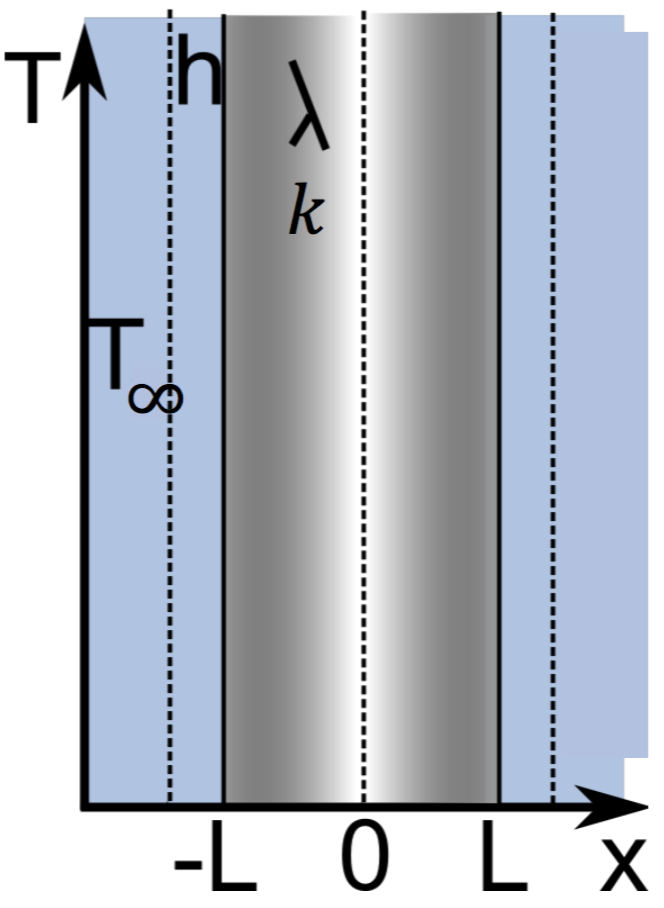
\includegraphics[scale=0.2]{ch4/6}
		\end{wrapfigure}	
		To describe that, we have to use the general equation again 
		\begin{equation}
			\frac{\partial T}{\partial t} + \alpha \frac{\partial ^2 T}{\partial x^2 }
		\end{equation}		 
	 	To that, we have to apply the boundary conditions :\\
	 	
	 	\begin{itemize}
	 		\item[•] no variation of temperature in the middle of the body : $ \frac{\partial T}{\partial x} = 0$ for $x = 0 \ \forall t \geq 0$
	 		\item[•] convection on the walls : $ -k\frac{\partial T}{\partial x} = h(T_L-T_\infty)$ for $|x| = L \ \forall t \geq 0$
	 		\item[•] initial temperature within the solid : $T = T_i$ for $t = 0 \ \forall -L < x < L$ \\
	 	\end{itemize}
	 	
	 	\begin{wrapfigure}[6]{r}{2.5cm}
		\vspace{-8mm}
		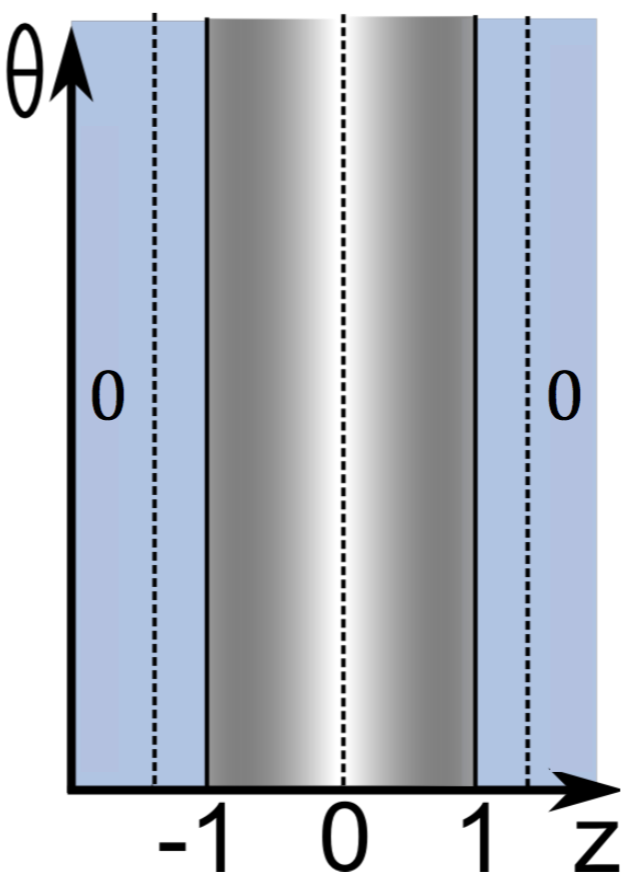
\includegraphics[scale=0.2]{ch4/7}
		\end{wrapfigure}	
	 	We transcript all that in a non-dimensional form by replacing $L$ by 1, $T$ by $\theta$, $T_i$ by 1, $t$ by $Fo$, $x$ by $X$ and the second condition becomes $- \frac{\partial \theta}{\partial X} = B_i \theta _1$ for $X = 1$ $\forall Fo \geq 0$. Where
	 	\begin{equation}
	 		\theta = \frac{T-T_\infty}{T_i-T_\infty} \qquad Fo = \frac{\alpha t}{L^2} \qquad X = \frac{x}{L} \qquad Bi = \frac{hL}{k}
	 	\end{equation}
	 	The solution of that (we don't calculate) is 
	 	\begin{equation}
	 		\theta = \sum _{i=1}^\infty \frac{2Bi \cos (\beta _i X)\exp (-\beta _i^2 Fo)}{\beta _i^2 (\beta _i^2 + Bi^2+Bi)}
	 	\end{equation}
	 	where the $\beta _i$ are the solutions of $\beta \tan (\beta ) = Bi$; these solutions are tabulated. 
	 	
		\begin{wrapfigure}[6]{l}{5.5cm}
		\vspace{-5mm}
		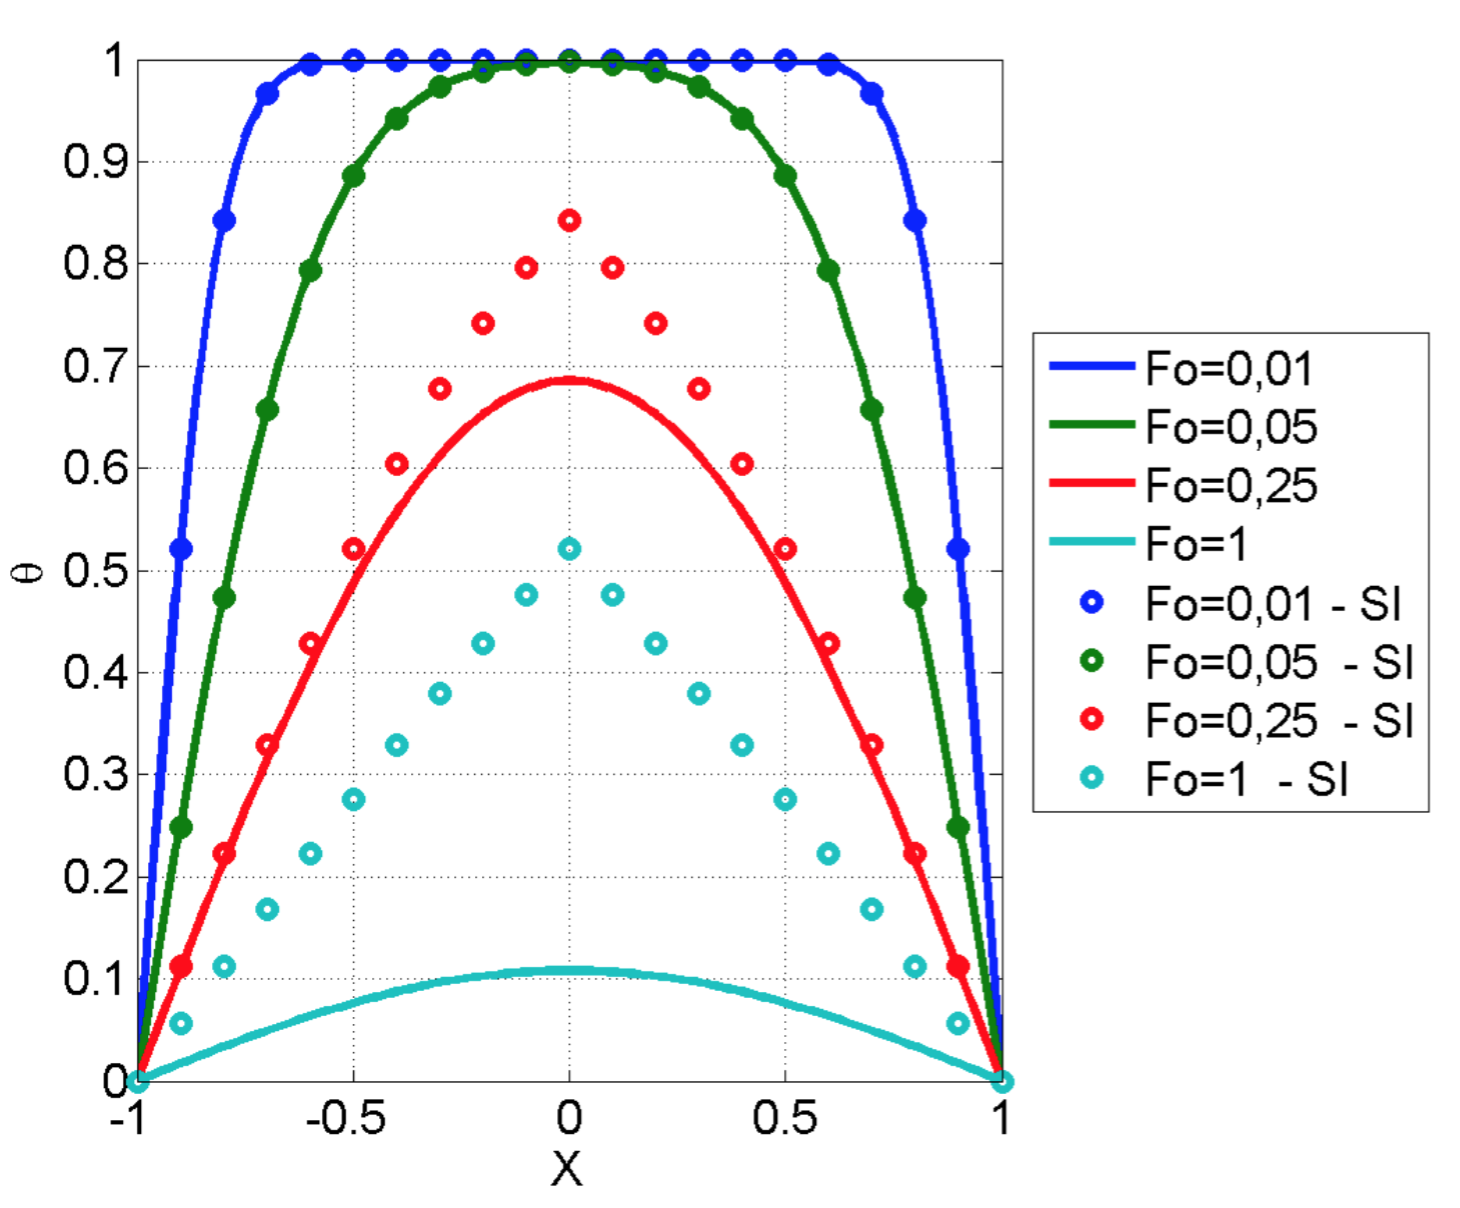
\includegraphics[scale=0.2]{ch4/8}
		\end{wrapfigure}	
	 	If we compare this case to the semi-infinite solid, we can see that the last theory is more precise when Fo number increases (time increase or length decrese).  It's similarly tabulate for the cylinder and the sphere. 